\documentclass[a4paper, oneside, 12pt, final, headsepline, footsepline]{scrartcl}
\usepackage{InfraAtHomeExportableArticle}

%------------ DOCUMENT -----------------
\begin{document}
%------------ HEADERS + FOOTERS --------
\configHeadersFooters
%------------ VARIABLES ----------------

\title{DMZ \\Pare-feu externe PFsense} % The short title appears at the bottom of every slide, the full title is only on the title page
\subtitle{Infr@home\_GUI-INST\_01-External-firewall}
\author{jmy37}
\date{\today}

%------------ TITLE PAGE -----------------
\maketitlepage

%------------ VERSIONNING ----------------
\section{Historique des versions}
\begin{table}[H]
    \centering
    % \begin{tabular}{|l|l|l|l|}
    \begin{tabular}{|>{\centering\arraybackslash}p{0.09\linewidth}|>{\centering\arraybackslash}p{0.12\linewidth}|>{\raggedright\arraybackslash}p{0.12\linewidth}|>{\raggedright\arraybackslash}p{0.6\linewidth}|}
        \hline
        \textbf{Version} & \textbf{Date} & \textbf{Auteur} & \textbf{Objet de la modification}                                              \\ \hline
        \textbf{1.0}     & 20/10/2020    & jmy37           & Création du document                                                           \\ \hline
        \textbf{1.1}     & 09/12/2020    & jmy37           & Ajout du serveur NTP (titre 5.7)                                               \\ \hline
        \textbf{2.0}     &               & jmy37           & Renommage du document pour séparer les pare-feu internes et externes           \\
                         &               &                 & Mise à jour de la licence vers FDL 1.3                                         \\
                         &               &                 & Ajout d'un disclaimer relatif aux choix des pare-feu (titre 2.1)               \\
                         &               &                 & Passage du routeur en UTC (titre 3)                                            \\
                         &               &                 & Ajout du layout français en console (titre 3)                                  \\
                         &               &                 & Ajout de la configuration (titre 4)                                            \\
                         &               &                 & Revue des alias et ruissellement dans la suite du document (titre 7.1)         \\
                         &               &                 & Création de l'annexe relative à la configuration des clients NTP (titre 8.1)   \\
                         &               &                 & Création de l'annexe relative aux alias du projet (titre 8.3)                  \\
                         &               &                 & Création de l'annexe relative aux règles du projet (titre 8.4)                 \\ \hline
    \end{tabular}
    \caption{Historique des versions}
    \label{tab:versioning}
\end{table}

%--------------------------- TABLE DES MATIÈRES -----------------------------
\newpage
\tableofcontents
\newpage

%--------------- DOCUMENT ----------------
\section{Préambule}
Ce document décrit l'installation, l'exploitation et la résolution de pannes associées au composant "Pare-feu externe" de la solution "Infr@home".\\

\subsection{Le projet PFsense}
PFsense est une solution de pare-feu s'appuyant sur le système d'exploitation FreeBSD. Le suivi du projet est assuré par la société Netgate. Le site \url{https://www.pfsense.org/} met à disposition le téléchargement des sources et de nombreuses documentations relatives au projet.

\begin{warning}
    Ce pare-feu est choisi dans le cadre du projet car il est disponible en sources ouvertes. Cependant, les deux pares-feux ne devraient pas être issus d'un même développement ; un pare-feu au moins devrait être un produit qualifié par l'ANSSI (idéalement le plus proche d'Internet).
\end{warning}

\subsection{Configuration requise}
La configuration minimale \footnote{\url{https://docs.netgate.com/pfsense/en/latest/book/hardware/minimum-hardware-requirements.html}} (trafic non-chiffré à 100Mo/s) pour PFsense est définie ci-dessous :
\begin{itemize}
    \item \textbf{Processeur} : 1 CPU monocore
    \item \textbf{Mémoire} : 1 Go de RAM
    \item \textbf{Stockage} : 20 Go d'espace disque
    \item \textbf{Réseau} : Au moins une interface par réseau soutenu
\end{itemize}

% Les performances requises peuvent être affinées en fonction des fonctionnalités à activer. Le détail des calculs est donné sur le site de PFsense\footnote{\url{https://docs.netgate.com/pfsense/en/latest/book/hardware/hardware-sizing-guidance.html#feature-considerations}}.
Les performances requises peuvent être affinées en fonction des fonctionnalités à activer. Le détail des calculs est donné sur le site de PFsense\footnote{\url{https://docs.netgate.com/pfsense/en/latest/book/hardware/hardware-sizing-guidance.html\#feature-considerations}}.\\
~\\
Il est ensuite nécessaire de récupérer la dernière image ISO de PFSense depuis le site de l'éditeur, en architecture x64 : \url{https://www.pfsense.org/download/}.\\
~\\
L'installation peut alors commencer.
\newpage
\section{Installation}
\subsection{Lancement de l'installation (depuis la console)}
Une fois la machine virtuelle créée, démarrer sur le DVD à jour. Laisser le système se lancer avec les options par défaut. Ensuite, suivre l'assistant d'installation :
\begin{itemize}
    \item Accepter les conditions d'utilisation (figure \ref{fig:03-install-console-01})
    \item Lancer l'installeur (figure \ref{fig:03-install-console-02})
    \item Définir l'interface WAN (figure \ref{fig:03-install-console-03})
    \item La configurer en DHCP (figure \ref{fig:03-install-console-04})
    \item Définir l'interface LAN (figure \ref{fig:03-install-console-05})
    \item Configurer son adresse IP et désactiver le DHCP (figure \ref{fig:03-install-console-06})
    \item Confirmer l'assignation des interfaces (figure \ref{fig:03-install-console-07})
    \item Valider l'emploi de la version communautaire (figure \ref{fig:03-install-console-08})
    \item Choisir le partitionnement par défaut (figure \ref{fig:03-install-console-09})
    \item Ne pas activer de RAID (figure \ref{fig:03-install-console-10})
    \item Confirmer le choix du disque (figure \ref{fig:03-install-console-11})
    \item Redémarrer
\end{itemize}

\begin{figure}[H]
    \centering
    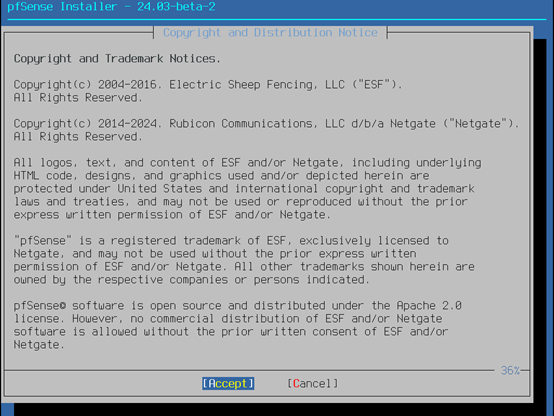
\includegraphics[width=0.88\textwidth]{03-Installation/Images/03-install-console-01.png}
    \caption{Installation - Conditions d'utilisation}
    \label{fig:03-install-console-01}
\end{figure}

\begin{figure}[H]
    \centering
    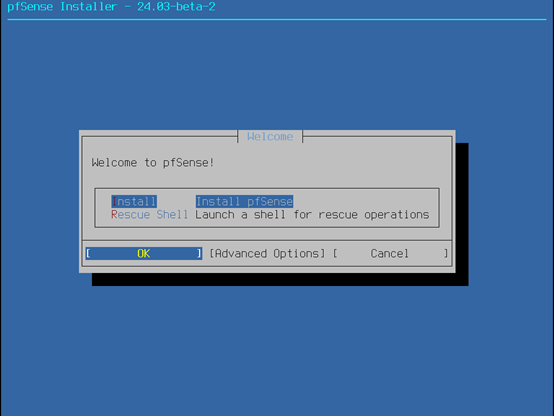
\includegraphics[width=0.88\textwidth]{03-Installation/Images/03-install-console-02.png}
    \caption{Installation - Lancement de l'installation}
    \label{fig:03-install-console-02}
\end{figure}

\begin{figure}[H]
    \centering
    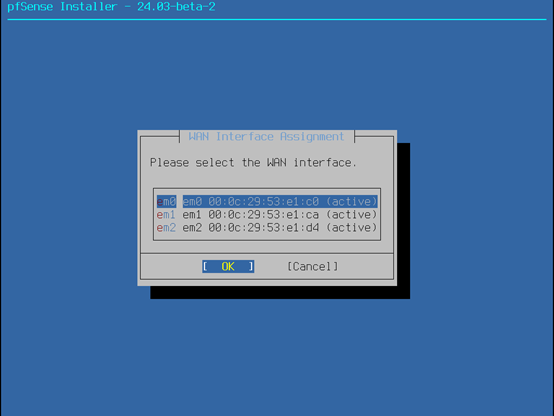
\includegraphics[width=0.88\textwidth]{03-Installation/Images/03-install-console-03.png}
    \caption{Installation - Attribution de l'interface WAN}
    \label{fig:03-install-console-03}
\end{figure}

\begin{figure}[H]
    \centering
    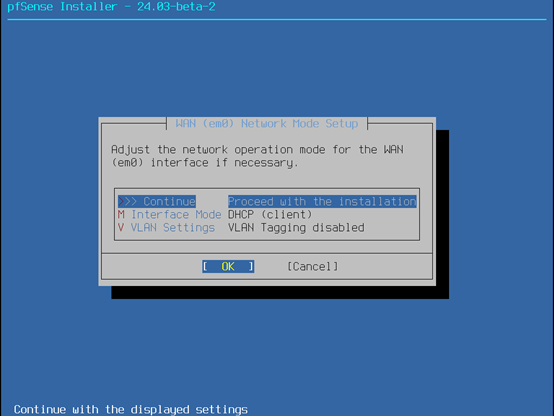
\includegraphics[width=0.88\textwidth]{03-Installation/Images/03-install-console-04.png}
    \caption{Installation - Configuration de l'interface WAN}
    \label{fig:03-install-console-04}
\end{figure}

\begin{figure}[H]
    \centering
    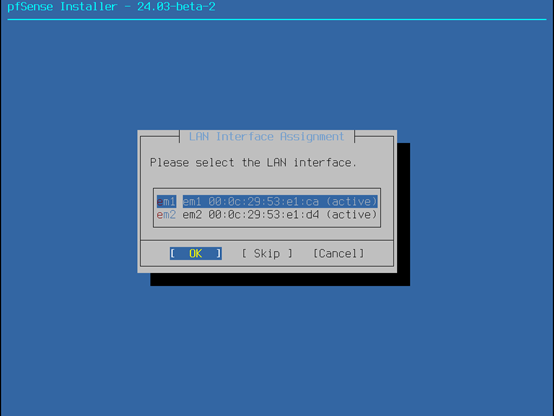
\includegraphics[width=0.88\textwidth]{03-Installation/Images/03-install-console-05.png}
    \caption{Installation - Attribution de l'interface LAN}
    \label{fig:03-install-console-05}
\end{figure}

\begin{figure}[H]
    \centering
    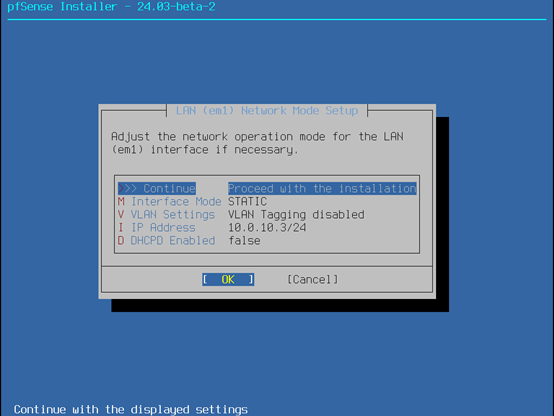
\includegraphics[width=0.88\textwidth]{03-Installation/Images/03-install-console-06.png}
    \caption{Installation - Configuration de l'interface LAN}
    \label{fig:03-install-console-06}
\end{figure}

\begin{figure}[H]
    \centering
    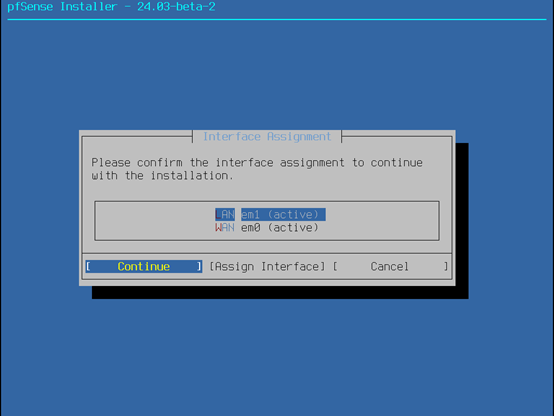
\includegraphics[width=0.88\textwidth]{03-Installation/Images/03-install-console-07.png}
    \caption{Installation - Validation de l'attribution des interfaces}
    \label{fig:03-install-console-07}
\end{figure}

\begin{figure}[H]
    \centering
    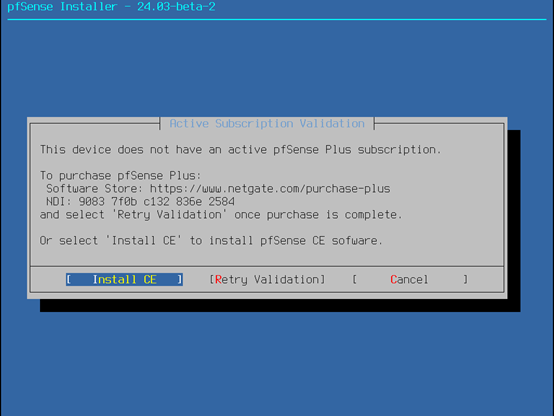
\includegraphics[width=0.88\textwidth]{03-Installation/Images/03-install-console-08.png}
    \caption{Installation - Choix de la souscription au support}
    \label{fig:03-install-console-08}
\end{figure}

\begin{figure}[H]
    \centering
    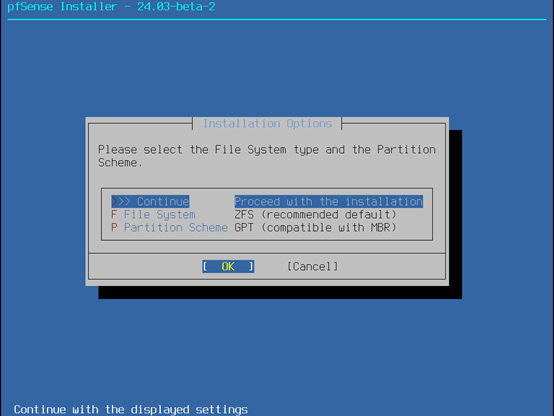
\includegraphics[width=0.88\textwidth]{03-Installation/Images/03-install-console-09.png}
    \caption{Installation - Choix du partitionnement}
    \label{fig:03-install-console-09}
\end{figure}

\begin{figure}[H]
    \centering
    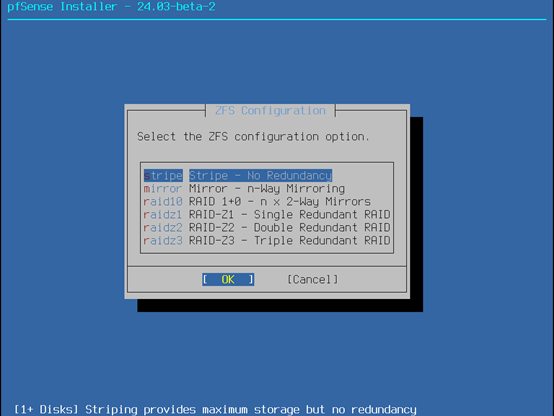
\includegraphics[width=0.88\textwidth]{03-Installation/Images/03-install-console-10.png}
    \caption{Installation - Configuration du RAID}
    \label{fig:03-install-console-10}
\end{figure}

\begin{figure}[H]
    \centering
    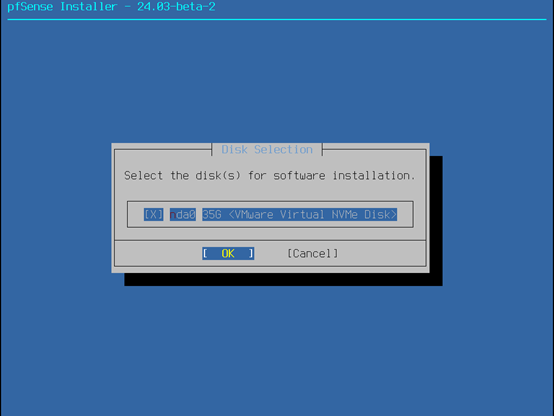
\includegraphics[width=0.88\textwidth]{03-Installation/Images/03-install-console-11.png}
    \caption{Installation - Choix du disque}
    \label{fig:03-install-console-11}
\end{figure}
\subsection{Configuration initiale (depuis la console)}
Une fois le serveur redémarré, il est nécessaire de lui attribuer ses adresses IP :
\begin{itemize}
    \item Choisir « 2 » pour assigner une adresse IP (figure \ref{fig:03-config-console-01})
    \item Choisir le numéro de l'adresse IP (figure \ref{fig:03-config-console-02})
    \item Choisir d'utiliser ou non DHCP (figure \ref{fig:03-config-console-03})
    \item Saisir l'adresse IP souhaitée (figure \ref{fig:03-config-console-04})
    \item Saisir le préfixe souhaité (figure \ref{fig:03-config-console-05})
    \item Saisir le masque désiré
    \item Ne pas définir de passerelle pour les réseaux locaux
    \item Procéder de la même manière pour l'IPv6
    \item Choisir d'activer le serveur DHCP ou non (figure \ref{fig:03-config-console-06})
    \item Ne pas activer le retour en http pour les connexions à l'interface d'administration (figure \ref{fig:03-config-console-07})
\end{itemize}

\begin{figure}[H]
    \centering
    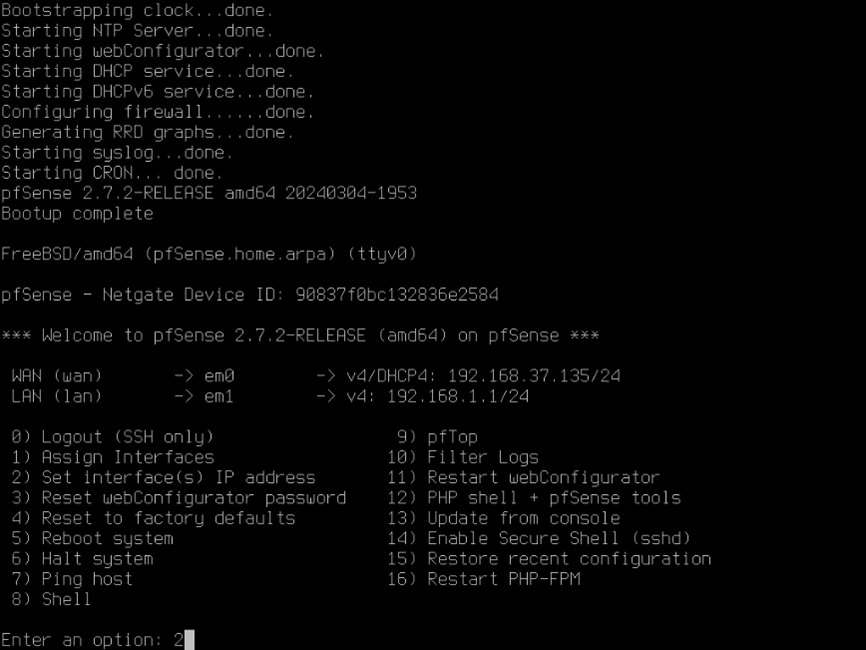
\includegraphics[width=0.88\textwidth]{03-Installation/Images/03-config-console-01.png}
    \caption{Configuration console - Choix de l'assignation d'adresses IP}
    \label{fig:03-config-console-01}
\end{figure}

\begin{figure}[H]
    \centering
    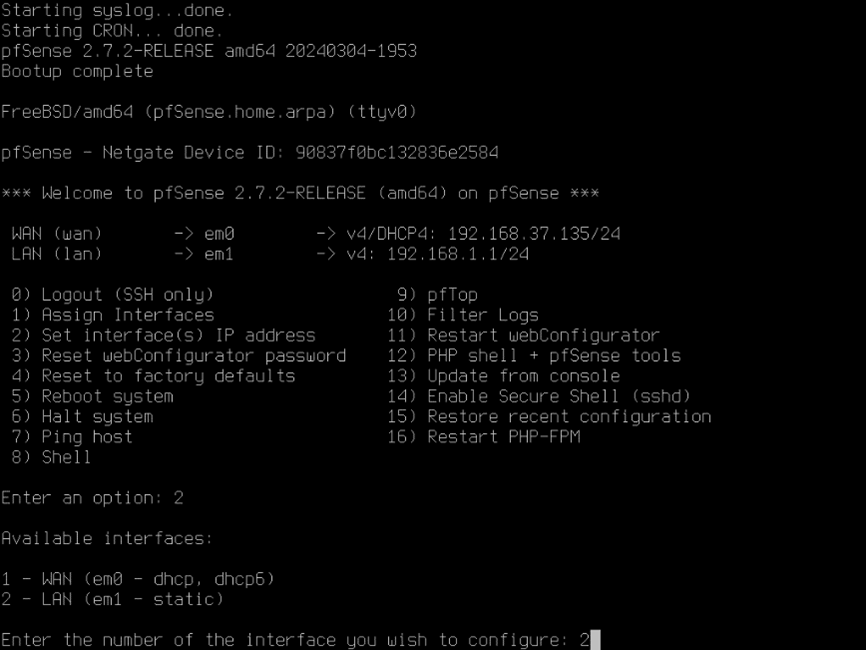
\includegraphics[width=0.88\textwidth]{03-Installation/Images/03-config-console-02.png}
    \caption{Configuration console - Choix de l'interface}
    \label{fig:03-config-console-02}
\end{figure}

\begin{figure}[H]
    \centering
    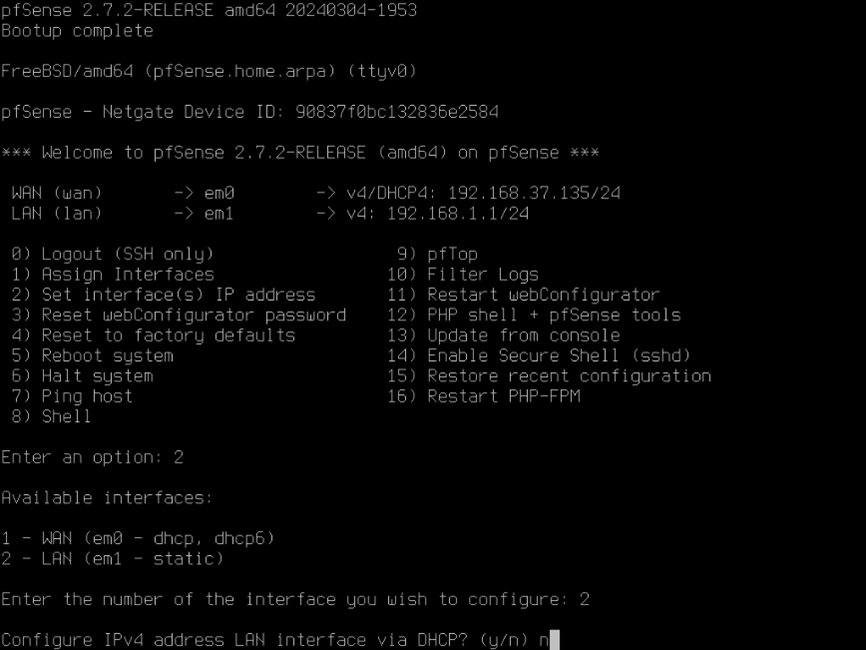
\includegraphics[width=0.88\textwidth]{03-Installation/Images/03-config-console-03.png}
    \caption{Configuration console - Choix de la non-utilisation de DHCP}
    \label{fig:03-config-console-03}
\end{figure}

\begin{figure}[H]
    \centering
    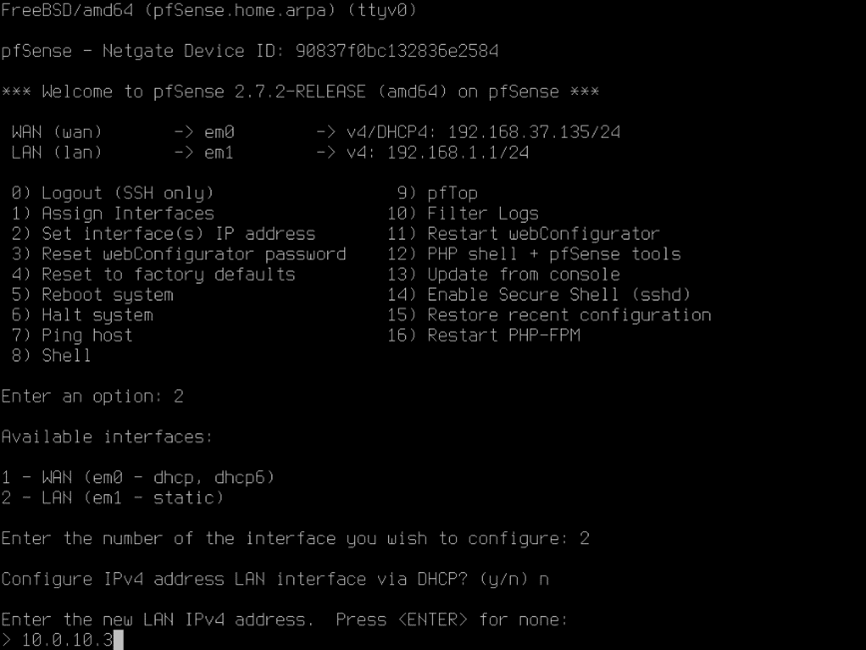
\includegraphics[width=0.88\textwidth]{03-Installation/Images/03-config-console-04.png}
    \caption{Configuration console - Définition de l'adresse IP}
    \label{fig:03-config-console-04}
\end{figure}

\begin{figure}[H]
    \centering
    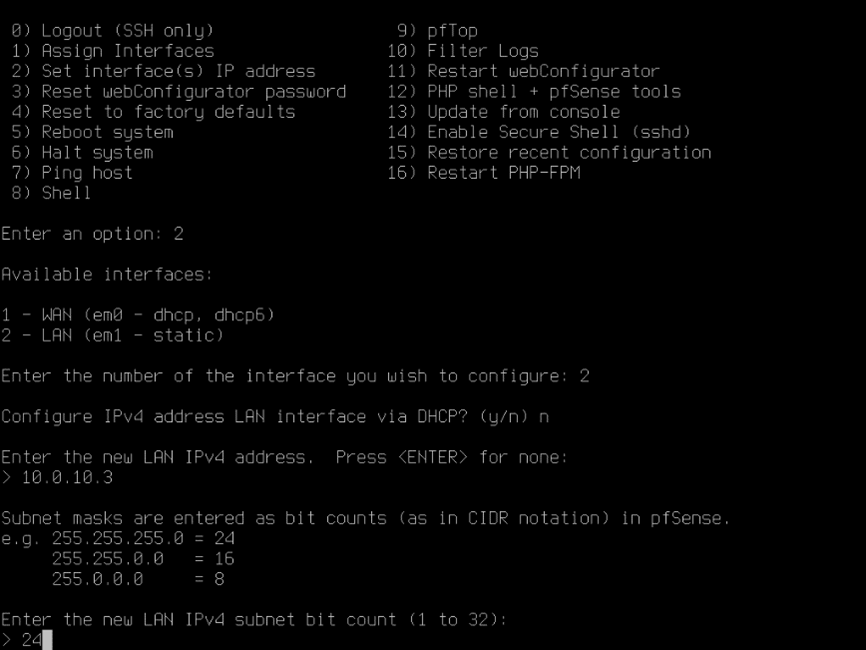
\includegraphics[width=0.88\textwidth]{03-Installation/Images/03-config-console-05.png}
    \caption{Configuration console - Définition du préfixe}
    \label{fig:03-config-console-05}
\end{figure}

\begin{figure}[H]
    \centering
    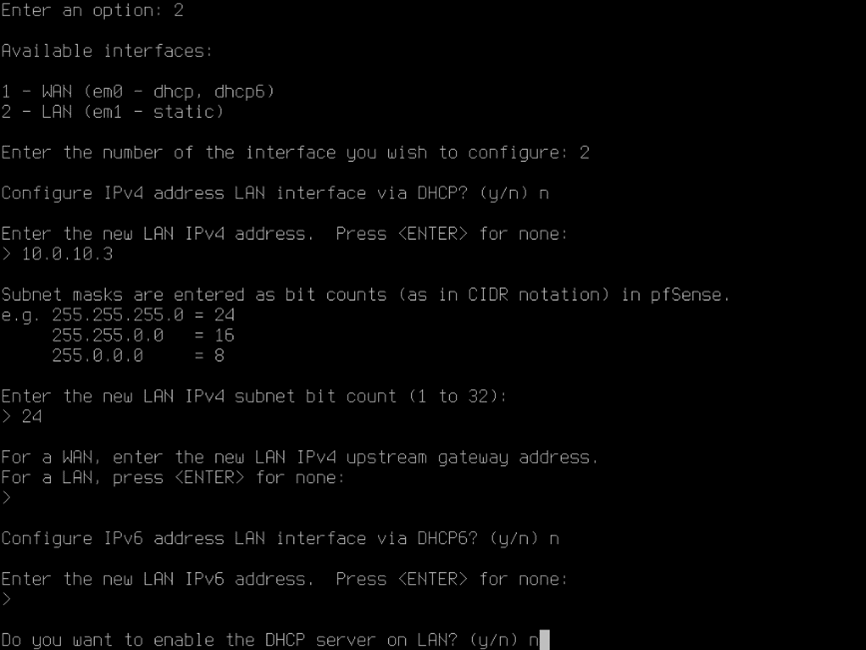
\includegraphics[width=0.88\textwidth]{03-Installation/Images/03-config-console-06.png}
    \caption{Configuration console - Non-activation du serveur DHCP}
    \label{fig:03-config-console-06}
\end{figure}

\begin{figure}[H]
    \centering
    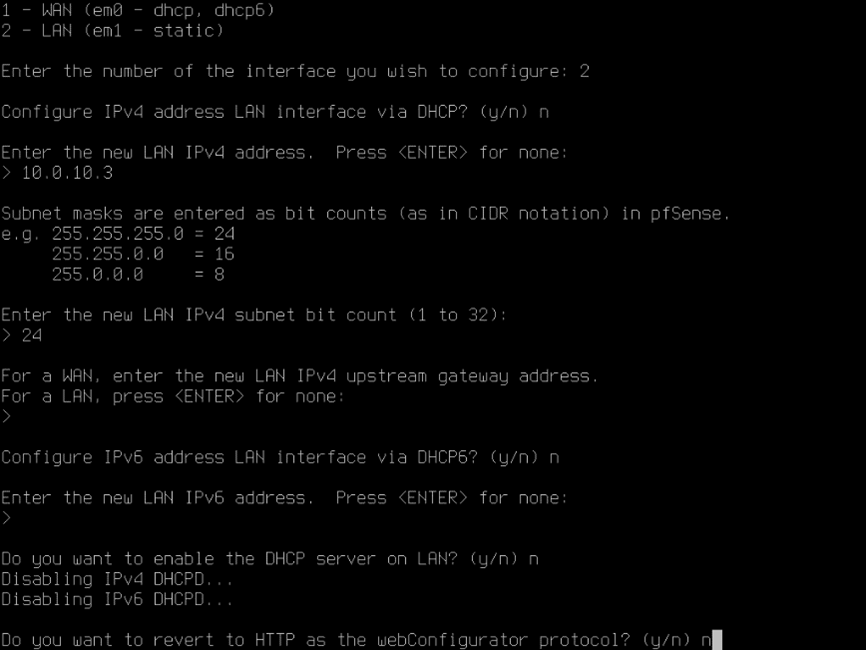
\includegraphics[width=0.88\textwidth]{03-Installation/Images/03-config-console-07.png}
    \caption{Configuration console - Non-activation du retour HTTP}
    \label{fig:03-config-console-07}
\end{figure}
\subsection{Configuration initiale (interface web)}
La suite de la configuration est réalisée au travers de l'interface web :
\begin{itemize}
    \item Se connecter à l'aide des identifiants par défaut (admin|pfsense)
    \item Lancer l'assistant de configuration initiale
    \item Choisir le nom d'hôte, le nom de domaine et les serveurs DNS (figure \ref{fig:03-config-web-01})
    \item Choisir un serveur NTP et un fuseau horaire ("Etc/UTC")
    \item Définir la configuration de l'interface WAN
    \item Définir la configuration de l'interface LAN
    \item Définir le mot de passe d'administration
    \item Recharger PFSense
    \item Accéder à "System/Package Manager"
    \item Accéder à "Available Package"
    \begin{itemize}
        \item Installer les additions invitées (uniquement pour un hyperviseur VMware) : "Open-VM-Tools"
        \item Installer la gestion du clavier "Shellcmd"
        \item Accéder à la configuration du service "Shellcmd" et ajouter la commande suivante (figure 13)
    \end{itemize}
\end{itemize}

\begin{lstlisting}[language=bash,caption={Définition du clavier français}]
kbdcontrol -l /usr/share/syscons/keymaps/fr.iso.kbd
\end{lstlisting}

\begin{figure}[H]
    \centering
    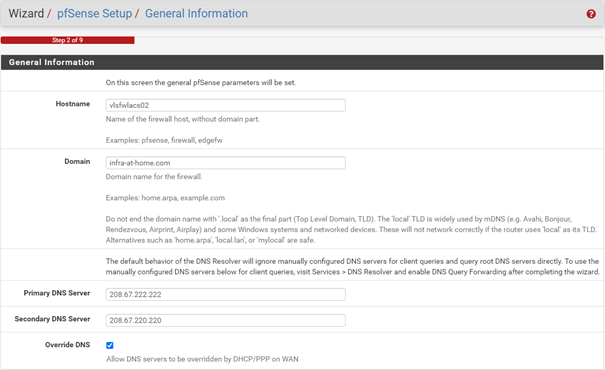
\includegraphics[width=1.0\textwidth]{03-Installation/Images/03-config-web-01.png}
    \caption{Configuration web - Nom d'hôte, de domaine et serveurs DNS}
    \label{fig:03-config-web-01}
\end{figure}

\begin{figure}[H]
    \centering
    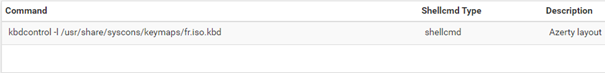
\includegraphics[width=1.0\textwidth]{03-Installation/Images/03-config-web-02.png}
    \caption{Configuration web - Configuration du clavier en disposition AZERTY}
    \label{fig:03-config-web-02}
\end{figure}

\begin{tip}
    Si la configuration est réalisée sur un réseau privé, il est important de permettre le trafic en provenance de réseaux privés sur l'interface WAN.
\end{tip}

\newpage
\section{Configuration}
\subsection{Configuration système avancée}
\subsubsection{Accès administrateur}
\begin{itemize}
    \item Désactiver l'autocomplétion du login dans l'interface web (figure \ref{fig:04-configuration-syst-adv-01})
    \item Activer la protection par mot de passe de la console (figure \ref{fig:04-configuration-syst-adv-02})
\end{itemize}

\begin{figure}[H]
    \centering
    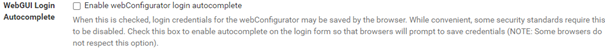
\includegraphics[width=1\textwidth]{04-Configuration/Images/04-configuration-syst-adv-01.png}
    \caption{Configuration - Avancé - Accès administrateur - Autocomplétion}
    \label{fig:04-configuration-syst-adv-01}
\end{figure}

\begin{figure}[H]
    \centering
    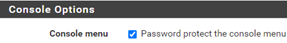
\includegraphics[width=0.5\textwidth]{04-Configuration/Images/04-configuration-syst-adv-02.png}
    \caption{Configuration - Avancé - Accès administrateur - Protection console}
    \label{fig:04-configuration-syst-adv-02}
\end{figure}

\subsubsection{Réseau}
\begin{itemize}
    \item Basculer sur le backend DHCP "Kea DHCP" (figure \ref{fig:04-configuration-syst-adv-03})
    \item Désactiver le trafic IPv6 (figure \ref{fig:04-configuration-syst-adv-04})
\end{itemize}

\begin{figure}[H]
    \centering
    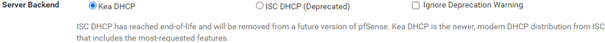
\includegraphics[width=1.0\textwidth]{04-Configuration/Images/04-configuration-syst-adv-03.png}
    \caption{Configuration - Avancé - Réseau - Backend DHCP}
    \label{fig:04-configuration-syst-adv-03}
\end{figure}

\begin{figure}[H]
    \centering
    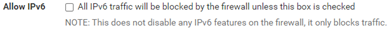
\includegraphics[width=0.7\textwidth]{04-Configuration/Images/04-configuration-syst-adv-04.png}
    \caption{Configuration - Avancé - Réseau - Blocage IPv6}
    \label{fig:04-configuration-syst-adv-04}
\end{figure}

\subsubsection{Divers}
\begin{itemize}
    \item Activer le mode MDS automatique (figure \ref{fig:04-configuration-syst-adv-05})
    \item Ne pas envoyer l'ID de périphérique Netgate (figure \ref{fig:04-configuration-syst-adv-06})
\end{itemize}

\begin{figure}[H]
    \centering
    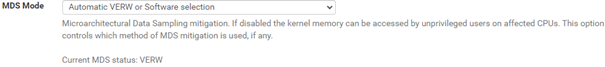
\includegraphics[width=1.0\textwidth]{04-Configuration/Images/04-configuration-syst-adv-05.png}
    \caption{Configuration - Avancé - Divers - MDS}
    \label{fig:04-configuration-syst-adv-05}
\end{figure}

\begin{figure}[H]
    \centering
    
\includegraphics[width=0.7\textwidth]{04-Configuration/Images/04-configuration-syst-adv-06.png}
    \caption{Configuration - Avancé - Divers - ID Netgate}
    \label{fig:04-configuration-syst-adv-06}
\end{figure}

\subsubsection{Notifications}
\begin{itemize}
    \item Désactiver les sons de la console (figure \ref{fig:04-configuration-syst-adv-07})
    \item Désactiver les bips de démarrage et d'extinction (figure \ref{fig:04-configuration-syst-adv-07})
\end{itemize}

\begin{figure}[H]
    \centering
    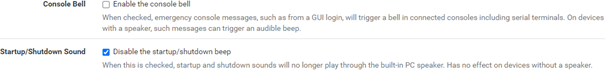
\includegraphics[width=1.0\textwidth]{04-Configuration/Images/04-configuration-syst-adv-07.png}
    \caption{Configuration - Avancé - Divers - ID Netgate}
    \label{fig:04-configuration-syst-adv-07}
\end{figure}
\subsection{Configuration générale}
\begin{itemize}
    \item Contrôler le nom d'hôte et de domaine (figure \ref{fig:04-configuration-generale-01})
    \item Renseigner les serveurs DNS et les noms d'hôtes associés (vérification TLS) (figure \ref{fig:04-configuration-generale-02})
    \item Renseigner le fuseau horaire et les serveurs de temps (figure \ref{fig:04-configuration-generale-03})
\end{itemize}

\begin{tip}
    Au moins trois références de temps devraient être utilisées. Les références suivantes peuvent être utilisées:
    \begin{itemize}
        \item \textbf{pool.ntp.org}
        \item \textbf{time.nist.gov}
        \item \textbf{time.google.com}
        \item \textbf{pfsense.pool.ntp.org}
        \item \textbf{time.windows.com}
    \end{itemize}
\end{tip}

\begin{figure}[H]
    \centering
    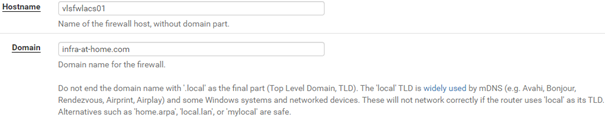
\includegraphics[width=1.0\textwidth]{04-Configuration/Images/04-configuration-generale-01.png}
    \caption{Configuration - Générale - Nom d'hôte et de domaine}
    \label{fig:04-configuration-generale-01}
\end{figure}

\begin{figure}[H]
    \centering
    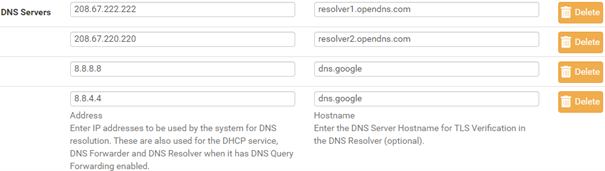
\includegraphics[width=1.0\textwidth]{04-Configuration/Images/04-configuration-generale-02.png}
    \caption{Configuration - Générale - Serveurs DNS}
    \label{fig:04-configuration-generale-02}
\end{figure}

\begin{figure}[H]
    \centering
    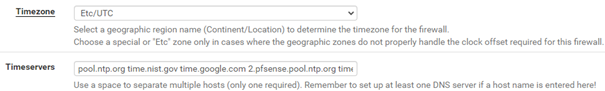
\includegraphics[width=1.0\textwidth]{04-Configuration/Images/04-configuration-generale-03.png}
    \caption{Configuration - Générale - Fuseau horaire et serveurs de temps}
    \label{fig:04-configuration-generale-03}
\end{figure}
\subsubsection{Mises à jour}
\begin{itemize}
    \item Réaliser une mise à jour depuis la branche stable si disponible
    \item Configurer le canal de mises à jour sur la dernière version stable (figure \ref{fig:04-configuration-updates-01})
    \item Maintenir actif le contrôle de mises à jour sur le dashboard (figure \ref{fig:04-configuration-updates-01})
\end{itemize}

\begin{tip}
    Ce dernier point peut être désactivé, notamment si le pare-feu n'aura pas accès à Internet.
\end{tip}

\begin{figure}[H]
    \centering
    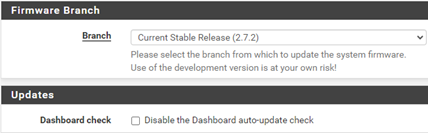
\includegraphics[width=0.7\textwidth]{04-Configuration/Images/04-configuration-updates-01.png}
    \caption{Configuration - Mises à jour}
    \label{fig:04-configuration-updates-01}
\end{figure}
\subsection{Interfaces}
\subsubsection{Assignation des interfaces}
Aucune interface ne doit être présente sur le serveur sans être assignée. Sur ce cluster, trois interfaces doivent être présentes :
\begin{itemize}
    \item \textbf{WAN}, l'interface directement connectée au routeur fournissant l'accès à Internet
    \item \textbf{DMZ}, l'interface connectée aux équipements présents en DMZ
    \item \textbf{FWLHA}, l'interface permettant aux pare-feu en cluster de communiquer ensemble, notamment en synchronisant les états et les configurations
\end{itemize}

\begin{warning}
    L'interface FWLHA doit idéalement être une connexion directe entre les équipements. En cas d'impossibilité, elle doit être sur un VLAN dédié et isolé, puisqu'elle fait circuler toutes les configurations et les états du cluster.
\end{warning}

\subsubsection{Interface WAN}
\begin{tip}
    Dans le cadre du projet, l'interface WAN sera configurée en DHCP, le routeur Internet fournissant les adresses IP dynamiquement.
\end{tip}

\begin{itemize}
    \item Activer l'interface (figure \ref{fig:04-configuration-interfaces-01})
    \item Nommer l'interface (figure \ref{fig:04-configuration-interfaces-01})
    \item Configurer l'adressage IPv4 (figure \ref{fig:04-configuration-interfaces-01})
    \item Configurer l'adressage IPv6 (figure \ref{fig:04-configuration-interfaces-01})
    \item Autoriser les adresses privées et de loopback (figure \ref{fig:04-configuration-interfaces-02})
    \item Bloquer le trafic bogon (adresses IP réservées mais ne respectant pas la RFC 1918\footnote{\url{https://datatracker.ietf.org/doc/html/rfc1918}} ou non-assignées) (figure \ref{fig:04-configuration-interfaces-02})
    \item Appliquer les changements
\end{itemize}

\begin{figure}[H]
    \centering
    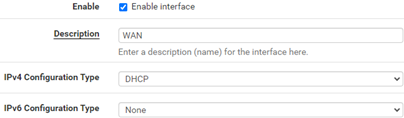
\includegraphics[width=0.7\textwidth]{04-Configuration/Images/04-configuration-interfaces-01.png}
    \caption{Configuration - Interfaces - WAN - Configuration générale}
    \label{fig:04-configuration-interfaces-01}
\end{figure}

\begin{tip}
    Dans le cadre du projet, le routeur opérateur fournit une adresse IP privée, impliquant la nécessité de permettre les adresses IP privées et de loopbacks à communiquer.
\end{tip}

\begin{figure}[H]
    \centering
    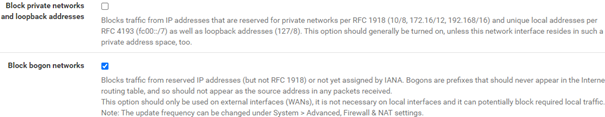
\includegraphics[width=1.0\textwidth]{04-Configuration/Images/04-configuration-interfaces-02.png}
    \caption{Configuration - Interfaces - WAN - Réseaux réservés}
    \label{fig:04-configuration-interfaces-02}
\end{figure}

\subsubsection{Interface DMZ}
\begin{itemize}
    \item Activer l'interface (figure \ref{fig:04-configuration-interfaces-03})
    \item Nommer l'interface (figure \ref{fig:04-configuration-interfaces-03})
    \item Configurer l'adressage IPv4 (figure \ref{fig:04-configuration-interfaces-03})
    \item Désactiver l'adressage IPv6 (figure \ref{fig:04-configuration-interfaces-03})
    \item Définir l'adresse IPv4 et son masque de sous-réseau (figure \ref{fig:04-configuration-interfaces-04})
    \item Autoriser les adresses privées et de loopback (figure \ref{fig:04-configuration-interfaces-05})
    \item Autoriser le trafic bogon (figure \ref{fig:04-configuration-interfaces-05})
    \item Appliquer les changements
\end{itemize}

\begin{figure}[H]
    \centering
    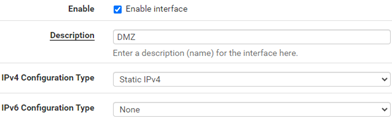
\includegraphics[width=0.7\textwidth]{04-Configuration/Images/04-configuration-interfaces-03.png}
    \caption{Configuration - Interfaces - DMZ - Configuration générale}
    \label{fig:04-configuration-interfaces-03}
\end{figure}

\begin{figure}[H]
    \centering
    
\includegraphics[width=1.0\textwidth]{04-Configuration/Images/04-configuration-interfaces-04.png}
    \caption{Configuration - Interfaces - DMZ - Adresse IPv4}
    \label{fig:04-configuration-interfaces-04}
\end{figure}

\begin{figure}[H]
    \centering
    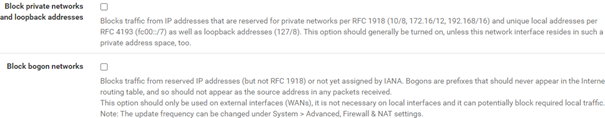
\includegraphics[width=1.0\textwidth]{04-Configuration/Images/04-configuration-interfaces-05.png}
    \caption{Configuration - Interfaces - DMZ - Réseaux réservés}
    \label{fig:04-configuration-interfaces-05}
\end{figure}

\subsubsection{Interface FWLHA}
\begin{itemize}
    \item Activer l'interface (figure \ref{fig:04-configuration-interfaces-06})
    \item Nommer l'interface (figure \ref{fig:04-configuration-interfaces-06})
    \item Configurer l'adressage IPv4 (figure \ref{fig:04-configuration-interfaces-06})
    \item Désactiver l'adressage IPv6 (figure \ref{fig:04-configuration-interfaces-06})
    \item Définir l'adresse IPv4 et son masque de sous-réseau (figure \ref{fig:04-configuration-interfaces-07})
    \item Autoriser les adresses privées et de loopback (figure \ref{fig:04-configuration-interfaces-08})
    \item Autoriser le trafic bogon (figure \ref{fig:04-configuration-interfaces-08})
    \item Appliquer les changements
\end{itemize}

\begin{figure}[H]
    \centering
    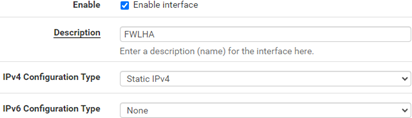
\includegraphics[width=0.7\textwidth]{04-Configuration/Images/04-configuration-interfaces-06.png}
    \caption{Configuration - Interfaces - FWLHA - Configuration générale}
    \label{fig:04-configuration-interfaces-06}
\end{figure}

\begin{figure}[H]
    \centering
    
\includegraphics[width=1.0\textwidth]{04-Configuration/Images/04-configuration-interfaces-07.png}
    \caption{Configuration - Interfaces - FWLHA - Adresse IPv4}
    \label{fig:04-configuration-interfaces-07}
\end{figure}

\begin{figure}[H]
    \centering
    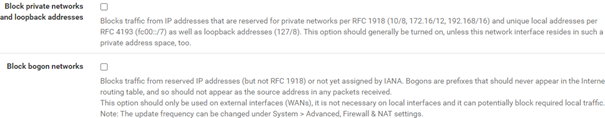
\includegraphics[width=1.0\textwidth]{04-Configuration/Images/04-configuration-interfaces-08.png}
    \caption{Configuration - Interfaces - FWLHA - Réseaux réservés}
    \label{fig:04-configuration-interfaces-08}
\end{figure}

\subsection{Passerelle}

Reprendre ici (page 26/53 du doc Word)
\subsubsection{Routage}

Reprendre ici (page 26/53 du doc Word)
\subsection{Serveur NTP}

Reprendre ici (page 27/53 du doc Word)
\subsection{Gestion des comptes locaux}

Reprendre ici (page 28/53 du doc Word)
\input{04-Configuration/Pages/Authent-ldap.tex}
\input{04-Configuration/Pages/Serveur-VPN-users.tex}
\subsection{Serveur VPN pour connexion intersite}
% \begin{tip}
%     Cette partie sera mise en oeuvre dans une version ultérieure du projet.
% \end{tip}

\begin{tip}
    \textcolor{Chartreuse4}{Cette partie sera mise en oeuvre dans une version ultérieure du projet.}
\end{tip}
\subsection{Sauvegarde du pare-feu}

Reprendre ici (page 30/53 du doc Word)

\end{document}